\documentclass{article}
%\usepackage{polski}
\usepackage{graphicx} 
\usepackage{tocloft}
\usepackage{amsmath}
\usepackage[a4paper, left=2cm, right=1cm, bottom=1in,top=2cm]{geometry}
\usepackage{fancyhdr}
\pagestyle{fancy}
\bibliographystyle{plain}

\fancyhf{}
%\setlength{\headheight}{15.2pt}

\lhead[]{\getcurrentref{} \leftmark}
\chead[]{Pendulum in physics}
\rhead[]{Michał Greczkowski}

\lfoot[]{}
\cfoot[]{}
\rfoot[]{\thepage}

\title{Pendulum in physics}
\label{maintitle}
\author{Michał Greczkowski}
\date{26.10.2023}
\begin{document}
\maketitle

\tableofcontents

\section{Introduction}
A pendulum is a device made of a weight suspended from a pivot so that it can swing freely. \textsuperscript{\cite{pendulum}} When a pendulum is displaced sideways from its resting, equilibrium position, it is subject to a restoring force due to gravity that will accelerate it back toward the equilibrium position. When released, the restoring force acting on the pendulum's mass causes it to oscillate about the equilibrium position, swinging back and forth. The time for one complete cycle, a left swing and a right swing, is called the period. The period depends on the length of the pendulum and also to a slight degree on the amplitude, the width of the pendulum's swing.
\begin{figure}[h]
 \centering
 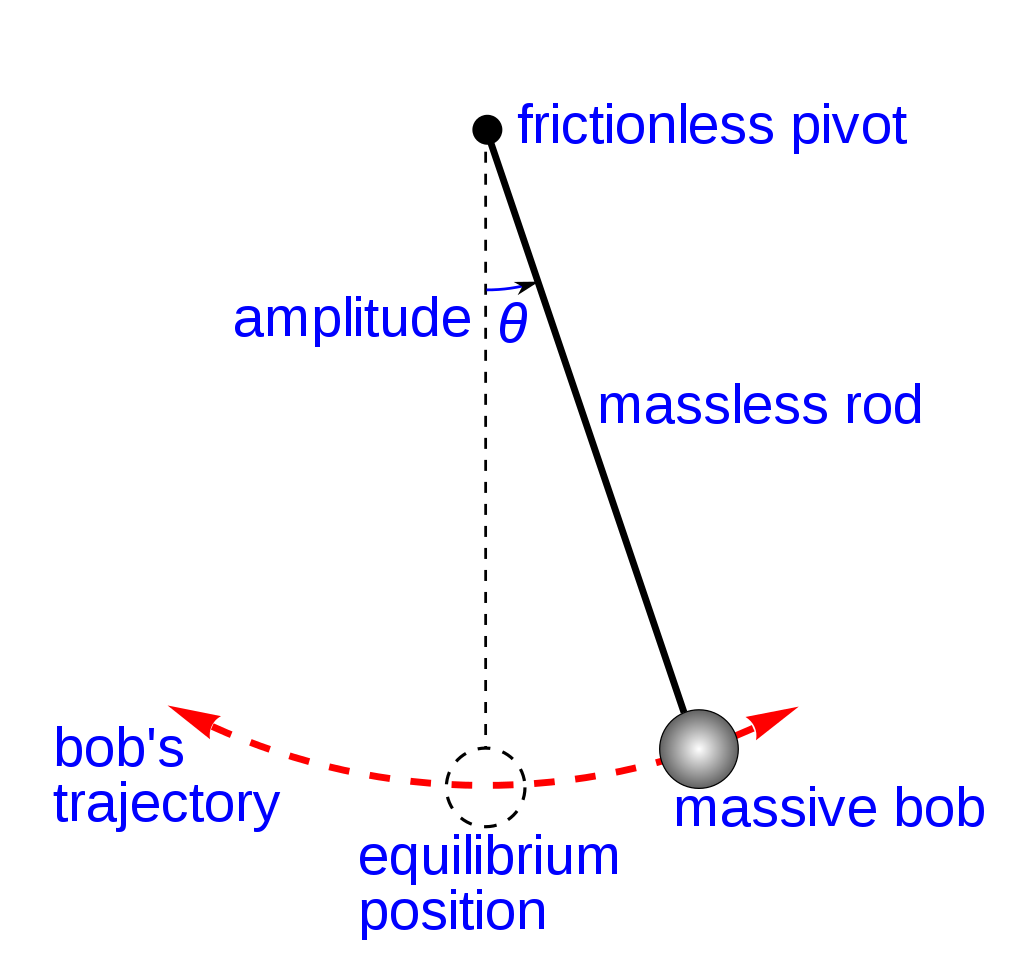
\includegraphics[scale=0.3]{pendulum.png}
 \caption{A simple pendulum model}
 \label{fig:pen}
\end{figure}
\section{Simple gravity pendulum}
The simple gravity pendulum is an idealized mathematical model of a pendulum. This is a weight (or bob) on the end of a massless cord suspended from a pivot, without friction. When given an initial push, it will swing back and forth at a constant amplitude. Real pendulums are subject to friction and air drag, so the amplitude of their swings declines.
An example model of such a pendulum was presented in Figure \ref{fig:pen}\\
Also for such a model Equation \ref{equ:first} is a very good approximation.
\newpage
\section{Equations}
Approximation of the period of oscillation
\begin{equation}
    T \approx 2\pi\sqrt{\frac{L}{g}}
\label{equ:first}
\end{equation}
Simple harmonic motion
\begin{equation}
\theta(t)=\theta_0\cos(\frac{2\pi}{T}t+\phi)
\end{equation}


\newpage
\section{Fun fact}
The regular motion of pendulums was used for timekeeping and was the world's most accurate timekeeping technology until the 1930s.\textsuperscript{\cite{2ndbook}}


\newpage

\section{Summary}
Pendulums are widely used in science education as an example of a harmonic oscillator, to teach dynamics and oscillatory motion. While they might look simple  they are a great way of showing physics phenomena and are a mighty educator for those starting with physics.
\vspace*{\fill}
\bibliography{bibliography}

\end{document}